\linespread{1.5}

Uma câmara frigorifica foi construído sobre um terreno cujo solo estava inicialmente à temperatura de $15ºC$. Quando a câmara passou a operar, à temperatura de $-35ºC$ o solo sob a câmara começou a resfriar por difusão de calor.
\begin{figure}[H]
    \centering
    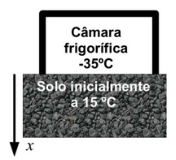
\includegraphics[width=0.3\linewidth]{fig/edp18.png}
    \label{fig:edp18}
\end{figure}
Admitindo que a temperatura do solo seja dada por:
\begin{equation}
\label{eq:edp18}
    u(x,t) = A + Berf\left(\frac{x}{2a\sqrt{t}}\right)
\end{equation}
sendo $x$ a profundidade em metros, $t$ o tempo em dias desde o inicio de operação da câmara e $a^2 = 0,075m^2/dia$, a difusividade térmica do solo, pede-se:
\begin{itemize}
    \item[a)] Determine as constantes $A$ e $B$ de modo que a equação \ref{eq:edp18} satisfaça a condição inicial $u(x,0) = 15ºC$, para $x>0$, e a condição de contorno $u(0,t) = -35ºC$, para $t>0$;
    \item[b)] Utilizando o resultado do item a), faça um esboço gráfico da temperatura do solo em função da profundidade para diferentes valores fixos do tempo;
    \item[c)]Calcule o tempo necessário para que a temperatura do solo baixe até $0ºC$ à profundidade de $50cm$, $1m$, e $2m$, respectivamente, abaixo da câmara frigorifica.
\end{itemize}
\begin{center}
        \textbf{Informação Útil}
        \textit{Função erro}
\end{center}
A função erro é definida por 
\begin{equation*}
    erf(z) = \frac{2}{\sqrt{\pi}}\int_0^z e^{-u^2}du
\end{equation*}
A função erro é ímpar e tende assintoticamente para $\pm1$ quando $z\rightarrow\pm\infty$. Abaixo, encontra-se uma tabela resumida da função erro:
\begin{table}[H]
\centering
\begin{tabular}{|c|c|}
\hline
z      & erf(z) \\ \hline
0.0000 & 0.0    \\ \hline
0.0889 & 0.1    \\ \hline
0.1791 & 0.2    \\ \hline
0.2725 & 0.3    \\ \hline
0.3708 & 0.4    \\ \hline
0.4769 & 0.5    \\ \hline
0.5951 & 0.6    \\ \hline
0.7329 & 0.7    \\ \hline
0.9062 & 0.8    \\ \hline
1.1631 & 0.9    \\ \hline
\end{tabular}
\end{table}